\section{Rigid Prototypes}
The goal of this research is to develop a flexible device but before delving into flexible prototypes we started by designing some rigid prototypes. The rigid prototypes were designed to test the concept of the device and to understand the limitations of the technology.

% -- Subsection 2.1
\subsection{1st version - Dresda Coils testbed}
The first prototype was designed to test the capabilities of the Dresden coils.
In the previous research done by the HZDR team \cite{HZDR} they tested the coil using a simple piece of flexible magnetic tape as a membrane.

\subsubsection{Flexible magnetic membrane}
This membrane is shaped like a "fish" so the tail can be fixed on a plane and the head can be free to bend up and down.

\begin{figure}
    \centering
    \resizebox{0.2\textwidth}{!}{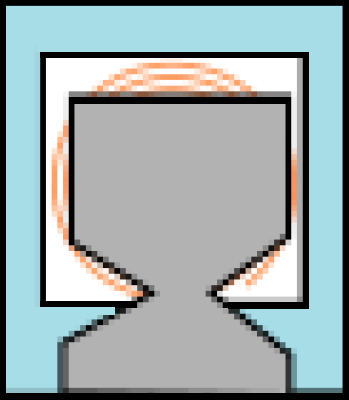
\includegraphics{Chapters/Chapter5/Rigid_Prototypes/Figures/Dresden_test.png}}
    \caption{Dresden coil HZDR test setup}
    \label{fig: Dresden_test}
\end{figure}

When the coil was powered, the magnetic field produced by the coil would repel the membrane and bend it up.
The coil would be powered with an AC signal at various frequencies, then one would need to keep his pulp suspended at a certain distance over the membrane and feel the vibration produced by the membrane.
The pulp needed to be suspended at a certain distance to avoid pressing on the membrane, this would have caused the membrane to stop vibrating.

\subsubsection{Adjustable height platform for coil and membrane}
The most important thing to solve was to find a way to keep the pulp at a certain distance from the membrane.
Firstly we designed a platform that could keep the finger steady.
\begin{figure}
    \centering
    \resizebox{0.5\textwidth}{!}{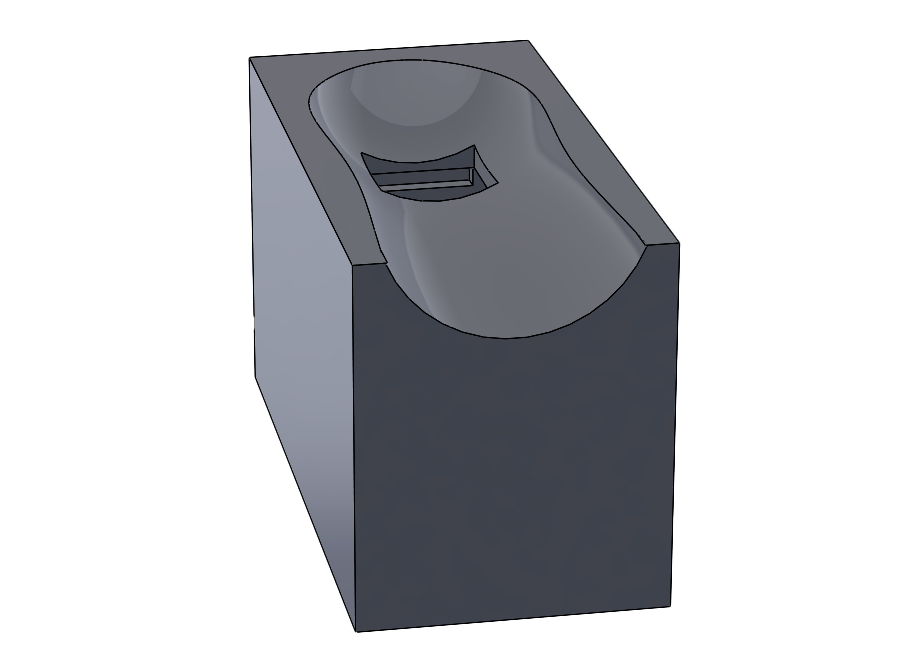
\includegraphics{Chapters/Chapter5/Rigid_Prototypes/Figures/finger_holder.png}}
    \caption{Finger platform}
    \label{fig: finger_platform}
\end{figure}

This platform was modeled to have an ergonomic cavity for the finger to rest in and a hole for the pulp to be suspended over the membrane.
The square hole is large enough to allow the "fish" membrane to move freely.
Under the hole, there is a large cavity where a mechanism is placed.
This mechanism is a platform where the coil and membrane can be placed in a configuration similar to the one used in the HZDR experiment.
The platform can then be raised or lowered to find the right distance between the membrane and the finger pulp.
\begin{figure}
    \centering
    \resizebox{0.5\textwidth}{!}{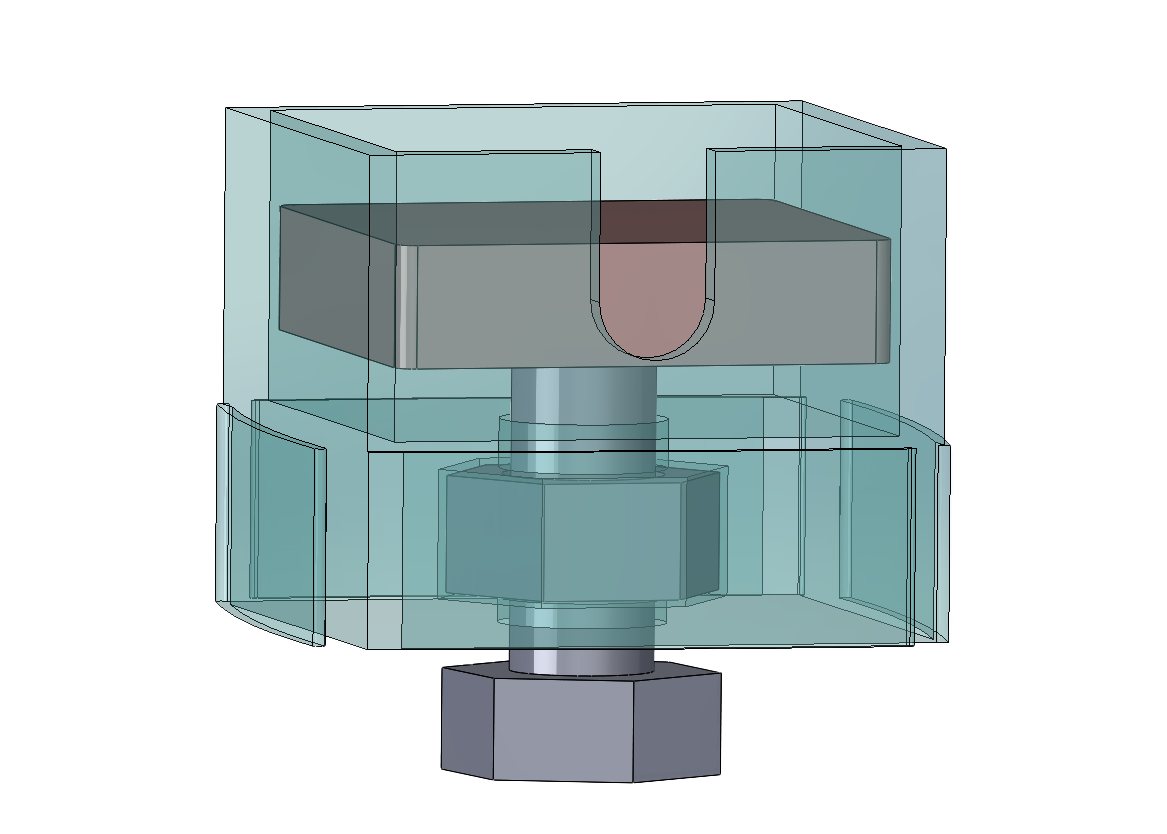
\includegraphics{Chapters/Chapter5/Rigid_Prototypes/Figures/adj_platform.png}}
    \caption{Adjustable platform}
    \label{fig: adj_platform}
\end{figure}
The mechanism is a simple screw that can be turned to raise or lower the platform.

\subsubsection{Prototype usability}
This prototype proved to be pretty finicky to use.
The main problem was that distance couldn't be easily adjusted as the platform wouldn't remain stable enough on the screw.
This meant that finding an optimal distance between the pulp and the membrane was difficult, especially because different people have different pulp thicknesses.
Even if a distance that was good for one person was found, the vibration produced by the membrane was very weak and could barely be felt.

% -- Subsection 2.2
\subsection{Wearable Rigid Prototypes}

\subsubsection{Finger-Membrane interface}

\subsubsection{Keep the distance from the coil}

\subsubsection{Heat dissipation}

